%
% This is the LaTeX template file for lecture notes for EE 382C/EE 361C.
%
% To familiarize yourself with this template, the body contains
% some examples of its use.  Look them over.  Then you can
% run LaTeX on this file.  After you have LaTeXed this file then
% you can look over the result either by printing it out with
% dvips or using xdvi.
%
% This template is based on the template for Prof. Sinclair's CS 270.

\documentclass[twoside]{article}
\usepackage{graphics}
\setlength{\oddsidemargin}{0.25 in}
\setlength{\evensidemargin}{-0.25 in}
\setlength{\topmargin}{-0.6 in}
\setlength{\textwidth}{6.5 in}
\setlength{\textheight}{8.5 in}
\setlength{\headsep}{0.75 in}
\setlength{\parindent}{0 in}
\setlength{\parskip}{0.1 in}
\usepackage{empheq}
\usepackage{graphicx}
\usepackage{wrapfig}
\usepackage[utf8]{inputenc}
\usepackage[english]{babel}

%
% The following commands set up the lecnum (lecture number)
% counter and make various numbering schemes work relative
% to the lecture number.
%
\newcounter{lecnum}
\renewcommand{\thepage}{\thelecnum-\arabic{page}}
\renewcommand{\thesection}{\thelecnum.\arabic{section}}
\renewcommand{\theequation}{\thelecnum.\arabic{equation}}
\renewcommand{\thefigure}{\thelecnum.\arabic{figure}}
\renewcommand{\thetable}{\thelecnum.\arabic{table}}

%
% The following macro is used to generate the header.
%
\newcommand{\lecture}[4]{
   \pagestyle{myheadings}
   \thispagestyle{plain}
   \newpage
   \setcounter{lecnum}{#1}
   \setcounter{page}{1}
   \noindent
   \begin{center}
   \framebox{
      \vbox{\vspace{2mm}
    \hbox to 6.28in { {\bf EE 382N: Distributed Systems
                        \hfill Fall 2017} }
       \vspace{4mm}
       \hbox to 6.28in { {\Large \hfill Lecture #1: #2  \hfill} }
       \vspace{2mm}
       \hbox to 6.28in { {\it Lecturer: #3 \hfill Scribe: #4} }
      \vspace{2mm}}
   }
   \end{center}
   \markboth{Lecture #1: #2}{Lecture #1: #2}
   %{\bf Disclaimer}: {\it These notes have not been subjected to the
   %usual scrutiny reserved for formal publications.  They may be distributed
   %outside this class only with the permission of the Instructor.}
   \vspace*{4mm}
}

%
% Convention for citations is authors' initials followed by the year.
% For example, to cite a paper by Leighton and Maggs you would type
% \cite{LM89}, and to cite a paper by Strassen you would type \cite{S69}.
% (To avoid bibliography problems, for now we redefine the \cite command.)
% Also commands that create a suitable format for the reference list.
\def\beginrefs{\begin{list}%
        {[\arabic{equation}]}{\usecounter{equation}
         \setlength{\leftmargin}{2.0truecm}\setlength{\labelsep}{0.4truecm}%
         \setlength{\labelwidth}{1.6truecm}}}
\def\endrefs{\end{list}}
\def\bibentry#1{\item[\hbox{[#1]}]}

%Use this command for a figure; it puts a figure in wherever you want it.
%usage: \fig{NUMBER}{SPACE-IN-INCHES}{CAPTION}
\newcommand{\fig}[3]{
			\vspace{#2}
			\begin{center}
			Figure \thelecnum.#1:~#3
			\end{center}
	}
% Use these for theorems, lemmas, proofs, etc.
\newtheorem{theorem}{Theorem}[lecnum]
\newtheorem{lemma}[theorem]{Lemma}
\newtheorem{proposition}[theorem]{Proposition}
\newtheorem{claim}[theorem]{Claim}
\newtheorem{corollary}[theorem]{Corollary}
\newtheorem{definition}[theorem]{Definition}
\newenvironment{proof}{{\bf Proof:}}{\hfill\rule{2mm}{2mm}}

% **** IF YOU WANT TO DEFINE ADDITIONAL MACROS FOR YOURSELF, PUT THEM HERE:

\begin{document}
%FILL IN THE RIGHT INFO.
%\lecture{**LECTURE-NUMBER**}{**DATE**}{**LECTURER**}{**SCRIBE**}
\lecture{}{Failures - November 3}{Vijay Garg}{Eric Addison}
%\footnotetext{These notes are partially based on those of Nigel Mansell.}

% **** YOUR NOTES GO HERE:

% Some general latex examples and examples making use of the
% macros follow.  
%**** IN GENERAL, BE BRIEF. LONG SCRIBE NOTES, NO MATTER HOW WELL WRITTEN,
%**** ARE NEVER READ BY ANYBODY.
\section{Introduction}
In this lecture, we continue our discussion of process failures. We know from the FLP result that in an asynchronous network, there is no algorithm that can solve the binary consensus problem in the presence of even one unannounced failure. We discuss here algorithms that can solve the consensus problem when we restrict ourselves to a synchronous network. Once that result is established, we broaden the failure model to allow arbitrary, or Byzantine, behavior.

\section{Synchronous Systems}
A synchronous distributed system is one in which there is some mechanism by which messages can time out. If a message takes longer than some specified time interval, the corresponding process can be considered as failed. A first attempt at solving the binary consensus problem in a synchronous network might be:
\begin{empheq}[box=\fbox]{align*}
P_i:: \quad &\\
& v_i - \text{ initial value}\\
& V - \text{ array of values received from others}\\
&\\
\textbf{do:}&\\
& \text{send $v_i$ to all}\\
& \text{receive $v_j$ from others, set $V[j] = v_j$}\\
& \text{decide on majority value in $V$}
\end{empheq}

Unfortunately, this algorithm does not work under certain failure conditions. For instance, consider three processes $P_1$,  $P_2$, and $P_3$, which propose values 1, 1, and 0 respectively, and agree to break ties by choosing 0. Imagine that $P_1$ successfully sends its value to $P_2$, but fails before it can send to $P_3$. The resulting $V$ arrays for $P_2$ and $P_3$ the look like:
\begin{align*}
    P_2: \> [1, 1, 0] \> \Rightarrow \text{choose 1}\\
    P_3: \> [x, 1, 0]  \> \Rightarrow \text{choose 0}
\end{align*}

This is clearly an incorrect state, as both remaining processes have confidently decided on different values. We can fix this issue by introducing the concept of \textit{rounds} that can last a finite duration.

\subsection{Binary Consensus}
We can think of performing the same algorithm stub above multiple times, where instead of broadcasting only your own value, you broadcast your entire vector $V$. By repeating this process a number of times, and merging a received vector with our own, we can ensure that eventually all processes will see the same vector of values and come to the same decision. This process must be done $f+1$ times in order to tolerate $f$ failures. The algorithm looks like:
\begin{empheq}[box=\fbox]{align*}
P_i:: \quad &\\
& V - \text{ array of known values}\\
&\\
\textbf{for }& round = 1..(f+1):\\
& \text{send $V$ to all}\\
& \textbf{for } j = 1..(N):\\
& \quad \text{receive $V_j$ from $P_j$}\\
& \quad V = V \cup V_j\\
\\
\text{decide} & \text{ on majority value in $V$}
\end{empheq}


\section{Byzantine Failures}
We can extend the failure model to encompass not just crashed processes, but faulty or even malicious processes by allowing a ``bad" process to generate arbitrary responses. In this so called Byzantine model, a faulty process can do whatever it wants, for example send an incorrect value, skip messages, etc.

\subsection{The Byzantine General Agreement Problem}

\begin{wrapfigure}{r}{0.25\textwidth}
    \centering
    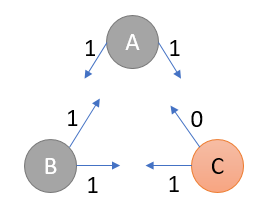
\includegraphics[scale=0.75]{images/Byz1}
    \caption{Faulty process $C$ causes the correct processes to disagree.}
    \label{fig:my_label}
\end{wrapfigure}

Consider the canonical allegory of three battalions of an army surrounding an enemy army. The battalions are led by Generals who must decide whether they will attack or retreat by coordinating with the other Generals. If the Generals all vote to attack, then they attack. If even one votes to retreat, then they all retreat. This problem is well modeled by the binary consensus problem, where instead of deciding on the majority value, the Generals decide on the minimum value. This is known as the Byzantine General Agreement Problem (BGA).

Let the processes (Generals) be labeled $A$, $B$, and $C$, where $C$ is a faulty process (treacherous General). The faulty process can cause the two correct processes to disagree by sending different information to each. For example, imagine that $A$ and $B$ both choose value 1 (attack), but the faulty process sends a 1 to one correct process, and a 0 to the other. This will cause the two correct processes to disagree, which in the context of the allegory, means that only one of the two battalions will attack, and presumably be defeated. 

What if we try to add multiple rounds to the process as with the simple failure model? It turns out that BGA cannot be solved, after any number of rounds, for $N=3$ and $f=1$, where $f$ is the number of faulty processes. This is a theorem:
\begin{align*}
    \text{\textbf{Theorem:} There is \textbf{no} protocol to solve BGA for $N=3$ and $f=1$}.
\end{align*}

\pagebreak
If $N=4$ and $f=1$, then it is solvable. This result can be proven, and generalized to the stronger result that:
\begin{align*}
    \text{\textbf{Theorem:} There is \textbf{no} protocol to solve BGA for $N \leq 3f$}.
\end{align*}


\subsection{The Queen Algorithm}
In 1989, Berman and Garay \cite{Berman:1989:AOD:646243.681443, Berman:1989:TOD:1398514.1398724} described two algorithms for solving the BGA problem, known as the King and Queen algorithms. The Queen algorithm is simpler and faster (requires fewer rounds), but the King algorithm can tolerate more failures. The queen algorithm is described below.

The Queen algorithm, also known as the rotating coordinator algorithm, can tolerate failures when $N > 4f$ and takes $f+1$ rounds. Initially, all processes store their value $x$ in their vector $V$ such that $V[i] = x$, and stores a default value $V[j]=v_\perp$ for all $j\neq i$. The algorithm now proceeds with $f+1$ rounds, each with two phases. In the first phase, all processes exchange their values $V[i]$ with all other processes. If there are no failures, all processes will now know the correct values, so each process now computes what would be the true chosen value if there were no failures and stores it as $v_i = majority(V)$, or $v_i = v_\perp$ if no majority is found. However we think there may be up to $f$ failures! In phase 2, a ``Queen", or coordinator, is assigned based on the round number, who sends her value out to all other processes. If a process's own value $v_i$ has an \textit{overwhelming majority}, that is, $tally(V,v_i) > N/2 + f$, then the process $P_i$ (re)sets the value $V[i] = v_i$. Otherwise, $P_i$ will set $V[i] = queenValue$.

Once an overwhelming majority is found, it persists (as shown in the text book). It can also be shown that a majority will be valid, and that agreement will be reached within the $f+1$ rounds. The algorithm is shown below.

\begin{empheq}[box=\fbox]{align*}
P_i:: \quad &\\
\textbf{var}&\\
& V: \text{ array of known values, initially } (V[i]=x)\> [j] = v_\perp, j \neq i\\
&\\
\textbf{for } & Q = 1..(f+1):\\
& \text{phase 1:}\\
& \quad \text{send $V[i]$ to all other processes}\\
& \quad \text{set $V[j]$ to the value received from all other $P_j$}\\
& \quad \text{$v_i = majority(V)$ or $v_\perp$ if no majority}\\
&\\
& \text{phase 2:}\\
& \quad \text{if}(Q==i):\\
& \quad \quad \text{send $v_i$ to all other processes}\\
& \quad \text{receive $queenValue$ from $P_Q$}\\
& \quad \text{if}(tally(V,v_i) > N/2+f:\\
& \quad \quad V[i] = v_i\\
& \quad \text{else } V[i] = queenValue\\
\text{decide } & y = V[i]
\end{empheq}


\bibliographystyle{unsrt}
\bibliography{refs}
\end{document}